\documentclass[final]{fhnwreport}       %[mode] = draft or final
                                        %{class} = fhnwreport, article, 
                                        %          report, book, beamer, standalone
%%---Main Packages-----------------------------------------------------------------------
\usepackage[english, ngerman]{babel}	%Mul­tilin­gual sup­port for LaTeX
\usepackage[T1]{fontenc}				%Stan­dard pack­age for se­lect­ing font en­cod­ings
\usepackage[utf8]{inputenc}				%Ac­cept dif­fer­ent in­put en­cod­ings
\usepackage{lmodern}                    %The newer Font-Set
\usepackage{textcomp}					%LaTeX sup­port for the Text Com­pan­ion fonts
\usepackage{caption}					%Customising captions in floating environments

\usepackage{graphicx} 					%En­hanced sup­port for graph­ics
\usepackage{float}						%Im­proved in­ter­face for float­ing ob­jects
\usepackage{ifdraft}                    %Let you check if the doc is in draft mode

%%---Useful Packages---------------------------------------------------------------------
\usepackage{color}						%Colour control for LaTeX documents
\usepackage[pdftex,dvipsnames]{xcolor}  %Driver-in­de­pen­dent color ex­ten­sions for LaTeX
\usepackage{csquotes}                   %Simpler quoting with \enquote{}
\usepackage{siunitx} 					%A com­pre­hen­sive (SI) units pack­age
\usepackage{listings}					%Type­set source code list­ings us­ing LaTeX
\usepackage[bottom]{footmisc}			%A range of foot­note op­tions
\usepackage{footnote}					%Im­prove on LaTeX's foot­note han­dling
\usepackage{verbatim}					%Reim­ple­men­ta­tion of and ex­ten­sions to LaTeX ver­ba­tim
\usepackage[textsize=footnotesize]{todonotes} %Mark­ing things to do in a LaTeX doc­u­ment
\usepackage{titling}					%Control over the typesetting of the \maketitle command

\usepackage{float}
\usepackage{wrapfig}

%%---Tikz Packages-----------------------------------------------------------------------
\usepackage{standalone}
\usepackage{tikz}
\usepackage{circuitikz}
\usetikzlibrary{arrows}
\usetikzlibrary{calc}
\usetikzlibrary{intersections}

%%---Math Packages-----------------------------------------------------------------------
\usepackage{amsmath}					%AMS math­e­mat­i­cal fa­cil­i­ties for LaTeX
\usepackage{amssymb}					%Type­set­ting symbols (AMS style)
%\usepackage{amstext}
%\usepackage{amsfonts}
%\usepackage{breqn}
\usepackage{array}						%Ex­tend­ing the ar­ray and tab­u­lar en­vi­ron­ments
\usepackage{amsthm}					%Type­set­ting the­o­rems (AMS style)

%%---Table Packages----------------------------------------------------------------------
\usepackage{tabularx}					%Tab­u­lars with ad­justable-width columns
%\usepackage{longtable}
\usepackage{multirow}					%Create tab­u­lar cells span­ning mul­ti­ple rows
\usepackage{multicol}					%In­ter­mix sin­gle and mul­ti­ple columns

%%---PDF / Figure Packages---------------------------------------------------------------
\usepackage{pdfpages}					%In­clude PDF doc­u­ments in LaTeX
\usepackage{pdflscape}					%Make land­scape pages dis­play as land­scape
\usepackage{subfig}					    %Fig­ures di­vided into sub­fig­ures

%%---Other Packages----------------------------------------------------------------------
%\usepackage{xargs}                     %De­fine com­mands with many op­tional ar­gu­ments


%%---Bibliography------------------------------------------------------------------------
\usepackage[style=ieee,urldate=comp,backend=biber]{biblatex}
\addbibresource{literature/bibliography.bib}

%%---Main Settings-----------------------------------------------------------------------
\graphicspath{{./graphics/}}			%Defines the graphicspath
\geometry{twoside=false}				    %twoside=false disables the "bookstyle"
\setlength{\marginparwidth}{2cm}
\overfullrule=5em						%Creates a black rule if text goes over the margins => debugging




%%---User Definitions--------------------------------------------------------------------
%%Tabel-Definitions: (requires \usepackage{tabularx})
\newcolumntype{L}[1]{>{\raggedright\arraybackslash}p{#1}}    %column-width and alignment
\newcolumntype{C}[1]{>{\centering\arraybackslash}p{#1}}
\newcolumntype{R}[1]{>{\raggedleft\arraybackslash}p{#1}}

%%---Optional Package Settings-----------------------------------------------------------
%Listings-Settings: (requires \usepackage{listings}) => Example with Matlab Code
\lstset{language=Matlab,%
    basicstyle=\footnotesize\ttfamily,
    breaklines=false,%
    morekeywords={switch, case, otherwise},
    keywordstyle=\color{Blue},%
    tabsize=2,
    %morekeywords=[2]{1}, keywordstyle=[2]{\color{black}},
    identifierstyle=\color{Black},%
    stringstyle=\color{Purple},
    commentstyle=\color{Green},%
    showstringspaces=false,%without this there will be a symbol in the places where there is a space
    numbers=left,%
    numberstyle={\tiny \color{black}},% size of the numbers
    numbersep=9pt, % this defines how far the numbers are from the text
    %emph=[1]{word1, word2,...},emphstyle=[1]\color{red}
}							

%Hurenkinder und Schusterjungen verhindern (kein Scherz, Google es)
\clubpenalty10000
\widowpenalty10000
\displaywidowpenalty=10000	



%Titel mit Mathematik immer fett drucken
\usepackage{sectsty}
\allsectionsfont{\boldmath}




			                %loads all packages, definitions and settings											
\title{Fachbericht}  		        %Project Title
\author{Team 1}      				    %Document Type => Technical Report, ...
\date{\today}          				   %Place and Date

\begin{document}

%%---TITLEPAGE---------------------------------------------------------------------------------
\thispagestyle{empty}
%	\ohead{\includegraphics[scale=0.5]{Bilder/Logo_FHNW.jpg}}
	\begin{figure}
		 \vspace*{-\topskip}\vspace*{-\headsep}
		
\includegraphics[scale=1]{graphics/fhnw_ht_logo_de.pdf}
	\end{figure}
	\begin{center}
		\vspace*{2cm}
		{\huge{\textbf{digitales Theremin}}}\\
		\vspace*{0.2cm}
		{\huge{\textbf{\thetitle}}}\\
		\vspace*{0.5cm}
		
		{\scshape\Large Projekt 5\\} \Large{\today}
		\vfill
		\begin{normalsize}
			{\begin{tabbing}
					\textbf{Auftraggeber:} \hspace{5cm}\= Prof. Dr. Hanspeter Schmid\\
					
					\\[0.8cm]
					\textbf{Betreuung:} 
					\>Prof. Dr. Hanspeter Schmid\\
					\>Herr Prof. Karl Schenk\\


					\\[0.8cm]
					\textbf{Team:} \>Andreas Frei \\ \>Dennis Aeschbacher \\ 

					\\[0.8cm]
					\textbf{Studiengang:} \>Elektro- und Informationstechnik
					\\[0.8cm]	\textbf{Semester:} \>Herbstsemester 2019
			\end{tabbing}}
		\end{normalsize}
		\vfill
	\end{center}
\clearpage
			
%%---ABSTRACT----------------------------------------------------------------------------
\selectlanguage{english}				%ngerman or english
\thispagestyle{empty}
\begin{abstract}
% Description aim/objective
\noindent In this Project a Theremin was built that mainly operates on digital hardware unlike the original device that solely used analog electronics. The device is supposed to be used in presentations for trade fairs by the Institute for Sensors and Electronics ISE. As such the device should be built in a appealing housing. Moreover the device should have other additional functionality such as soundeffects or the ability to record sound.
% Method
The digital hardware was implemented in VHDL on the developer board DE1-SoC from terasIC with a Cyclone V FPGA from Intel. The sole analog component implemented was the oscillator that controls the pitch. 
% Results
The pitch of the device can be changed well, but the sound itself has a flaw at the moment, because there is an audible crackle. This is due to a communication problem with the codec that was used for the audio output. This problem will not be corrected during this project, because the communication will be implemented differently in the finished product.
% Conclusion
The work in this project served as a platform for the continuation in project 6. The next steps would be to implement the volume control and redesign the pcb for two antennas and oscillators.


\end{abstract}	



%%---TABLE OF CONTENTS-------------------------------------------------------------------
\pagenumbering{Roman}		
\selectlanguage{ngerman}				%ngerman or english
\tableofcontents
\clearpage

%%---TEXT--------------------------------------------------------------------------------
\pagenumbering{arabic}
\clearpage
\section{Einleitung}\label{sec:Einleitung}
Das Theremin kennen heutzutage nur wenige Leute, obwohl es das erste elektronische Instrument war. Es wurde 1920 von dem Russen Lev Sergejewitsch Termen, welcher sich später zu Leon Theremin umbenennen liess, erfunden \cite{Theremin_h}. Personen die regelmässig Filme schauen, haben die Musik welche mit einem Theremin gemacht wird bestimmt schon einmal gehört. Ein Beispiel dafür ist Ghostbusters, wo das Theremin oft im Hintergrund zu hören ist. Zudem ist das Theremin in einigen Science-Fiction-Filmen und Horrorfilmen zu hören \cite{Goast_m}. Das Theremin wird ohne es zu berühren gespielt, indem man mit den Händen die Distanz zu zwei Antennen ändert. Dies führt zu Veränderung der Tonhöhe und Lautstärke.

Im Projekt 5 und 6 soll nun ein solches Instrument entwickelt werden. Mit dem Unterschied, dass das sonst analoge Instrument digital aufgebaut werden soll. Dabei soll es auf einem Field Programmable Gate Array (FPGA) implementiert werden. Später soll das Theremin als Messeobjekt für das Institut für Sensorik und Elektronik ISE verwendet werden. Im Rahmen des Projekt 5 wurde die Tonhöhenantenne des Theremin realisiert. Dazu wurde die Antenne zusammen mit dem Antennenoszillator analog beibehalten. Die restlichen Komponenten wurden in VHDL realisiert. Das Resultat wurde auf dem DE1-SoC Board von terasIC mit einem Cyclone V FPGA von Intel getestet.

Der folgende Fachbericht beginnt mit dem Kapitel \ref{sec:Technische Grundlagen} Technische Grundlagen.In der ersten Hälfte des Kapitel wird erklärt wie ein analoges Theremin funktioniert und welche Komponenten ein Theremin ausmachen. In der zweiten Hälfte werden digitale Lösungsansätze besprochen. Anschliessend wird im Kapitel \ref{sec:Realisierung} Realisierung beschrieben wie die Komponenten realisiert wurden. Im Kapitel \ref{sec:Validierung} Validierung wird als erstes auf die Inbetriebnahme des Antennenoszillators eingegangen. Als nächstes werden die Simulationen des VHDL Codes erläutert. Im letzten Abschnitt wird auf die Inbetriebnahme des VHDL Codes auf dem DE1-SoC Board Bezug genommen.






\pagebreak

	
\clearpage
\section{Technische Grundlagen}\label{sec:Technische Grundlagen}
Um ein Verständnis für dessen Funktionsweise zu gewinnen, ist in diesem Kapitel als erstes erklärt, wie ein analoges Theremin funktioniert. Anschliessend folgt ein kleiner Abschnitt zur Musiktheorie. Zuletzt werden verschiedene Algorithmen erklärt, welche im digitalen Theremin eingesetzt wurden.
	\subsection{analoges Theremin}\label{subsec:Theremin_analog}
Das klassische Theremin besitzt zwei Antennen. Der Spieler kann über die senkrecht angebrachte Antenne  die  Tonhöhe beeinflussen. Mit der waagrechten Antenne beeinflusst der Spieler die Lautstärke. Eine typische Eigenschaft des Theremin ist, dass der Ton des Theremin in einem weitem Frequenzbereich kontinuierlich veränderbar ist. Das Theremin kann daher alle Frequenzen in einem Bereich spielen, im Gegensatz zu den meisten anderen Instrumenten.

Der Spieler spielt das Theremin durch verstimmen der Oszillatoren über die Antennen.
Die Hand des Spielers verändert über die jeweilige Antenne die Schwingfrequenz des Tonhöhen und Lautstärkeoszillators. Dabei wird der kapazitive Anteil des LC-Schwingkreises beeinflusst, was eine Änderung der Schwingfrequenz zur Folge hat. 
Die Frequenz dieser Oszillatoren ist jedoch weit über dem hörbaren Bereich (zwischen \SI{100}{kHz} bis \SI{1}{MHz}). Mit Hilfe eines Mischers und einem Referenzoszillator wird die Frequenzdifferenz des Tonhöhenoszillators hörbar gemacht und danach verstärkt\cite{Franzis}. Der Lautstärkepegel ergibt sich durch die Verwendung eines Bandpassfilters und nachfolgenden Hüllkurvendetektor. Die Abbildung \ref{img:Blockschaltbild_analog} gibt einen Überblick über die Schaltungskomponenten eines Theremins. Die einzelnen Schaltungsteile sind im folgenden Teil genauer erklärt.

\begin{figure}[h]
	\centering
	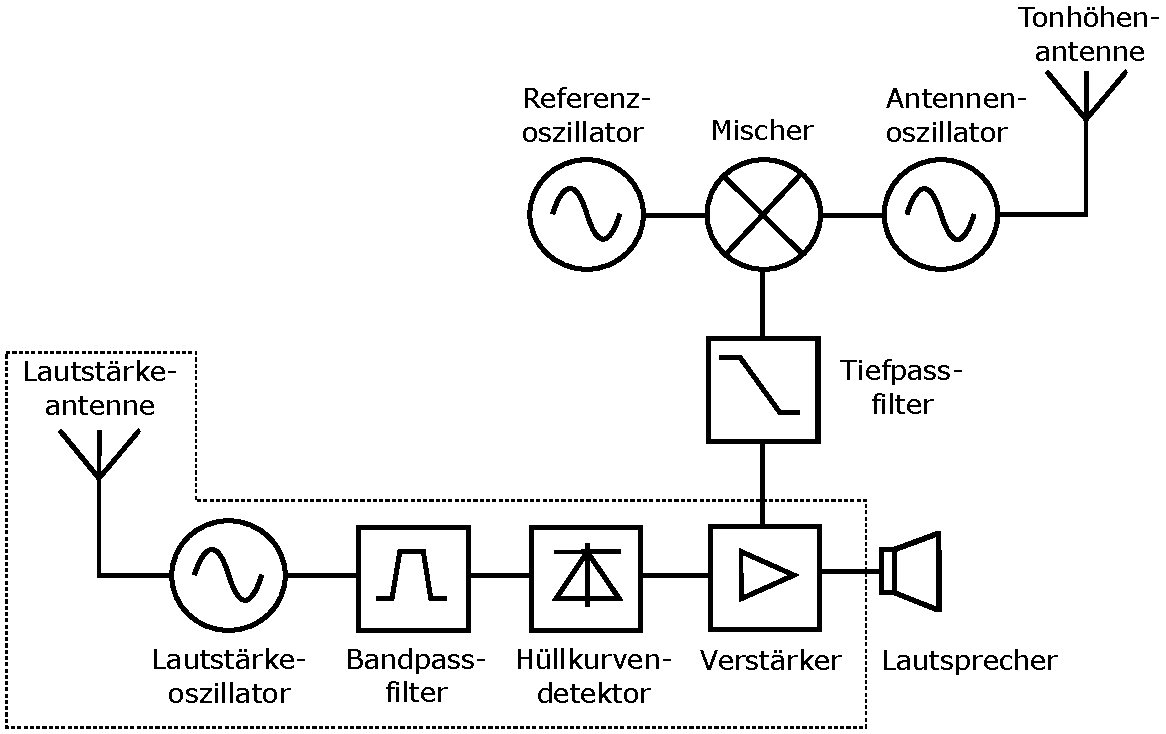
\includegraphics[width=0.8\textwidth]{Blockschaltbild_analog.pdf}
	\caption{Blockschaltbild eines analogen Theremins}
	\label{img:Blockschaltbild_analog}
\end{figure}

\paragraph{Tonhöhenoszillator und Tonhöhenantenne}\mbox{}\\

Die Tonhöhenantenne ist ein Metallrohr welches mit dem Tonhöhenoszillator verbunden ist.
Der Spieler kann über die Distanz seiner Hand zur Antenne die Frequenz des Tonhöhenoszillator verändern. Die über die Antenne zu erreichende Kapazitätsänderung ist sehr gering. Diese liegt im Picofarad Bereich \cite{physik_theremin}.Die Grundfrequenz des Tonhöhenoszillator muss weit über dem hörbaren Bereich liegen, dass eine genügend grosse Frequenzänderung entsteht.

\paragraph{Lautstärkeoszillator und Lautstärkeantenne}\mbox{}\\ 

Die Lautstärkeantenne ist wie die Tonhöhenantenne ein Metallrohr, welches mit dem Lautstärkeoszillator verbunden ist. Die durch den Spieler beeinflusste Frequenzänderung wandelt ein Hüllkurvendetektor in eine Spannung um. Diese Spannung dient dem Verstärker als Steuergrösse um das Audio Signal zu verstärken. \cite{Franzis}. 

\paragraph{Mischer und Referenzoszillator}\mbox{}\\ 
\\Die erzeugte Frequenz der Tonhöhenantenne ist weit über dem vom Menschen hörbaren Bereich. Der Mischer multiplizeirt die Signale des Referenzoszillators und des Tonhöhenoszillators wie in Formel \ref{equ:mischer}. $A_1\sin(\omega_1)$ ist das Signal des Referenzoszillators und $A_2\sin(\omega_2)$ das Signal des Tonhöhenoszillators.

\begin{equation}
V_{out} = A_{1}A_{2} \sin(\omega_{1}t)   \sin(\omega_{2}t) 
\label{equ:mischer}
\end{equation}

$V_{out}$ kann durch Additionstheoreme umgeformt werden. Dabei erhält man folgenden Ausdruck:

\begin{equation}
V_{out} = A/2[\cos((\omega_{1}-\omega_{2})t)  - \cos((\omega_{1}+\omega_{2})t) ]
\label{equ:mischer_trigo}
\end{equation}

Das Ausgangssignal $V_{out}$ hat zwei Frequenzkomponenten. Zum einen die Differenz der beiden Frequenzen zum anderen die Summe der Frequenzen. Dabei ist bei dem Theremin nur die Differenz der Frequenzen von Interesse \cite{physik_theremin}.

Eine Kalibration des Theremins ist vor jedem Gebrauch nötig. Es könnte beispielsweise sein, dass die Differenz der Frequenz ausserhalb des hörbaren Bereiches ist. Dazu stellt der Spieler beim klassischen Theremin mit Hilfe eines Trimmkondensators am Referenzoszillator die Differenzfrequenz auf \SI{0}{Hz} ein.

\paragraph{Tiefpassfilter}\mbox{}\\ 
\\Das Tiefpassfilter filtert die hochfrequente Komponente aus Formel \ref{equ:mischer_trigo} weg. Übrig bleibt die Differenz der Oszillatorfrequenzen. Dieser ist der interessante Anteil des Mischprozesses, da er im hörbaren Bereich ist.
\begin{equation}
V_{out} = A/2cos((\omega_{1}-\omega_{2})t) 
\label{equ:mischer_gefilt}
\end{equation}

\paragraph{Verstärker und  Lautsprecher}\mbox{}\\ 
\\Der Verstärker verstärkt das Ausgangssignal des Tiefpassfilter abhängig von der Spannung, welche vom Hüllkurvendetektor stammt.

	\subsection{digitales Theremin}\label{subsec:Theremin_digital}

bla bla







\clearpage
\section{Realisierung}\label{sec:Realisierung}

Das digitale Theremin ist auf dem Entwicklungsboard DE1-SoC von Terasic aufgebaut. Dieses enthält ein Cyclone V 5CSEMA5 FPGA von Intel. Weiter befindet sich auf dem Board der Audio Codec WM8731 von Wolfson für die Ausgabe an einem Lautsprecher. In Abbildung \ref{img:Blockschaltbild_top} ist der Aufbau des digitalen Theremin aufgezeigt inklusive der Peripherie ausserhalb des FPGA.\\
Das Theremin, welches im FPGA aufgebaut ist, besteht aus zwei Bereichen. Einerseits der Signalverarbeitung und Übermittlung an den Codec. Dieser besteht aus den Komponenten \textit{Lautstärken}- und \textit{Tonhöhenverarbeitung}, \textit{DC-FIFO} und dem \textit{Audioserialisierer}. Der zweite Bereich ist das Nios II System. Dieses besteht aus dem Prozessor und diversen IP Cores, welche die Kommunikation mit den Peripherien ermöglicht. Ausserhalb des FPGA befindet sich zudem das entwickelte PCB, welches die beiden Antennenoszillatoren enthält und das Spielen des Theremins ermöglicht.\\
Die Kommunikation zwischen dem Nios II Prozessor und den anderen Komponenten geschieht über das \textit{Avalon Memory Mapped Interface}. Der Prozessor agiert in dieser Kommunikation als Master und die restlichen Komponenten als Slaves. Die Übertragung der Audioinformation in der Signalverarbeitung geschieht über das \textit{Avalon Streaming Interface}. Wobei Sender als Streaming Source und Empfänger als Streaming Sink deklariert sind. Das Streaming Interface ist notwendig für den Einsatz des Dual-Clock-FIFO (DC-FIFO). Dieses übernimmt den Übergang verschiedener Clockregionen zwischen den Komponenten \textit{Tonhöhenverarbeitung} und \textit{Audioserialisierer}.\\
Die Clocks, welche zu den verschiedenen Komponenten führen sind in Abbildung \ref{img:Blockschaltbild_top} für eine bessere Übersichtlichkeit weggelassen worden. Für eine Liste aller Clock Frequenzen und deren Ziel siehe Kapitel \ref{subsec:Clock}.

\begin{figure}[h!]
	\centering
	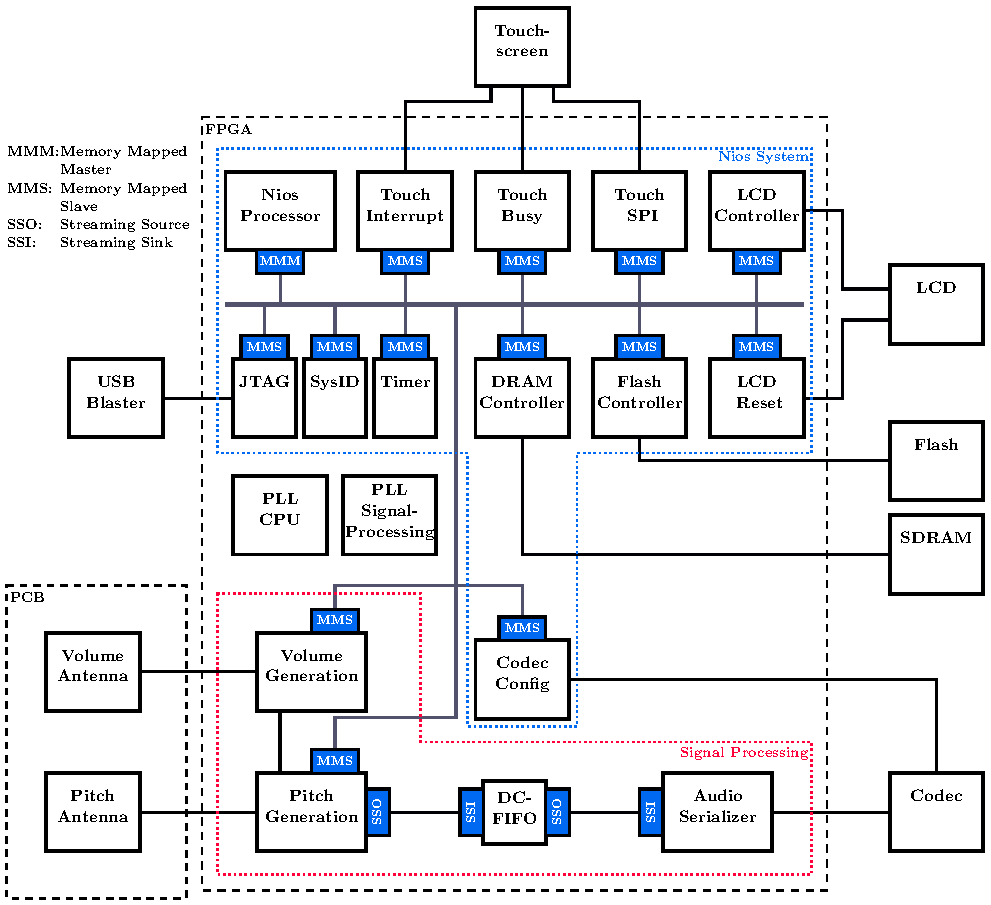
\includegraphics[width=1\textwidth]{Blockschaltbild_top.pdf}
	\caption{Blockschaltbild gesammtes Theremin} 
	\label{img:Blockschaltbild_top}
\end{figure}  

\clearpage


	\subsection{Tonhöhen- und Lautstärkenoszillator}\label{subsec:Antennenoszilator}
Für die Antennenoszillator-Schaltung haben wir uns im Projekt 5 für den Colpitts-Oszillator aus Abbildung \ref{img:colpitts} entschieden. Der Aufbau im Projekt 5 umfasste nur einen Oszillator zur Veränderung der Tonhöhe.

Es handelt sich dabei um einen Colpitts-Oszillator mit einem JFET. Diese Schaltung ist von dem Bauset ''Theremin selber bauen`` von Franzis übernommen \cite{Franzis}. 
Da der im Bauset verwendete JFET nicht mehr bestellbar ist, war ein Wechsel auf den J113 N-Kanal JFET nötig. Die mit LTspice simulierten Werte des J113 glichen stark der Originalschaltung, weshalb der Entscheid auf diesen fiel. 
Damit das Sinussignal des Antennenoszillator nicht A/D gewandelt werden muss, wandelt eine Komparatorschaltung das Sinussignal in ein Rechtecksignal mit gleicher Frequnez um. 
Diese ist mit \SI{3.3}{V} betrieben, da die Logikeingänge des FPGA auf diese Spannung ausgelegt sind. 

Im Projekt 5 wurde als Antenne ein Messingrohr verwendet. Diese ist am Anschluss pitch\_antenna verbunden. 

Die Ausgangsspannung des Colpitts-Oszillator ist über den Kondensator C11 entkoppelt. Dies entfernt den DC-Anteil. Der Kondensator C11 und die Widerstände R3 und R4 bilden zusammen einen Hochpass. Damit die Oszillatorfrequenz von ca \SI{562}{kHz} das Filter passieren kann, ist C11 so gewählt, dass die Grenzfrequenz des Filters bei ca \SI{265}{kHz} liegt. 

Auf dem PCB sind nun im Projekt 6 zwei solche Oszillatoren verbaut: Der Tonhöhenoszillator und der Lautstärkenoszillator. Das PCB ist mit einem \SI{12} {VDC} Schaltnetzteil gespiessen. Der MC7809 Spannungsregler generiert die \SI{9} {VDC} für die Colpitts-Oszillatorschaltungen. Die \SI{3.3} {VDC} für den Komperator erzeugt der LT1117 Spannungsregler. Bei der Wahl der Spannungsregler ist darauf geachtet worden, dass die erzeugten Spannungen möglichst störungsfrei ist und wenig Ripple aufwiesen. Das gesamte Schema der Schaltung ist im Anhang enthalten.

\begin{figure}[h]
	\centering
	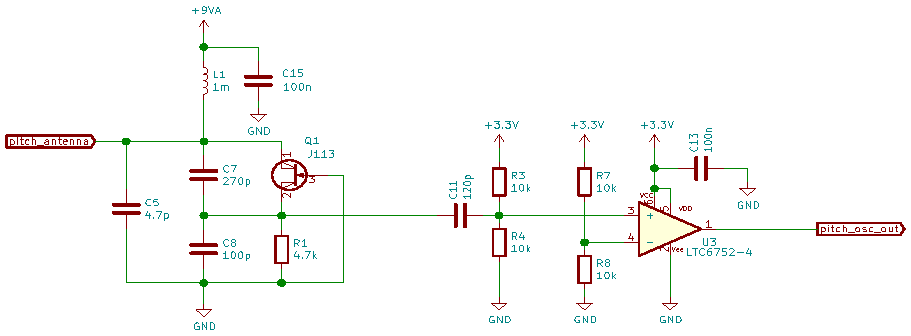
\includegraphics[width=\textwidth]{colpitts.pdf}
	\caption{Schema Antennenoszillator. Links Collpitts-Oszillator, rechts Komparatorschaltung}
	\label{img:colpitts}
\end{figure} 

\clearpage



	\input{sections/3_2_Referenzoszillator}
	\input{sections/3_3_Mischer}
	\input{sections/3_4_Filter}
	\input{sections/3_5_Tongenerierung}

\pagebreak

\clearpage
\section{Validierung}\label{sec:Validierung}
In diesem Kapitel wird zuerst das Antennenoszillator PCB getestet. Anschliessend wird mit Simulationen des VHDL Codes, durch berechnen der jeweiligen Spektren der Zwischenresultate, deren gesamte Funktion getestet. Zum Schluss wird auf die Inbetriebnahme und das Debugging Bezug genommen.
	\subsection{PCB}\label{subsec:PCB}
bla bla


	\input{sections/4_2_Simulation}
	\input{sections/4_3_Debugging}
\pagebreak


\clearpage
\section{Schlusswort}\label{sec:Schlusswort}
Im Rahmen des Projekt 5  wurde eine digitale Plattform für die Verarbeitung von Signalen einer Thereminantenne entwickelt. Alle Komponenten ausser der Antennenoszillator wurden in VHDL realisiert. Die VHDL Komponenten wurden so realisiert, dass diese im Projekt 6 weiter gebraucht werden können.
Momentan lässt sich das Theremin ohne Lautstärkeantenne spielen. Über zwei Taster kann der digitale Referenzoszillator manuell auf die Frequenz des Tonhöhenoszillator abgestimmt werden. Sobald das Theremin kalibriert ist kann es Töne von ca. 100-2000Hz spielen. 
Die Ziele welche in der Projektklärung definiert wurden konnten erfüllt werden. Bei der kontinuierlichen Tongenerierung gibt es noch eine Unschönheit bei der Ansteuerung des Codec. Es ist im generierten Ton ein Knacken zu hören, welches auf einen Fehler in der Ansteuerung des verwendeten Codec zurückzuführen ist. Dieser Fehler besteht nach wie vor. Jedoch wird diese Ansteuerung in Projekt 6 sowieso anders realisiert.

Im Projekt 6 wird die zweite Antenne implementiert, um gleichzeitig die Lautstärke einstellen zu können. Des weiteren soll es möglich sein diskrete Töne zu spielen. Dieser Modus soll es Anfängern ermöglichen bekannte Melodien nachspielen zu können. \\
Damit das theoretische Wissen aus dem Fach digitale Schaltungstechnik (dst) in die Praxis umgesetzt werden kann, wird ein Nios Soft Core Prozessor implementiert. Dieser übernimmt die Ansteuerung des Codec und die Modus Verwaltung. Beim starten des Theremin soll ein automatisches Tuning des Referenzoszillators stattfinden. Dazu wird der digitale Referenzoszillator auf die Frequenz des Antennenoszillator abgestimmt. Um das Theremin für Messen zu verwenden wird das DE1-SoC Board und die Antennenoszillatoren mit den Antennen in ein ansprechendes Gehäuse verbaut. Die Antennen sollen abgeschraubt werden können um einen komfortablen Transport zu ermöglichen.

Als erstes wird im Projekt 6 mit der Implementierung der Lautstärkeantenne auf dem FPGA und dem Redesign des PCB begonnen. Zudem muss Recherche in das Thema Nios Soft Core Prozessor angestellt werden, um diesen später implementieren zu können. 







\pagebreak

\section{Ehrlichkeitserklärung}\label{sec:Ehrlichkeitserklärung}
Mit der Unterschrift bestätigen die Unterzeichnenden Teammitglieder, dass die vorliegende Projektdokumentation selbstständig im Team und ohne Verwendung anderer, als der angegebenen Hilfsmittel verfasst wurde, sämtliche verwendeten Quellen erwähnt und die gängigen Zitierregeln eingehalten wurden. Eine Überprüfung der Arbeit auf Plagiate mithilfe elektronischer Hilfsmittel darf vorgenommen werden.


\vspace{20mm}


\begin{center}
		\renewcommand{\arraystretch}{1}
	\begin{tabular}{lp{5em}l} 
  
		
		Unterschrift:   && Ort, Datum: \\
		&&\\
		\hspace{5cm}   && \hspace{5cm} \\\cline{1-1}\cline{3-3}
		&&\\
		&&\\
		Unterschrift:   && Ort, Datum: \\
		&&\\
		\hspace{5cm}   && \hspace{5cm} \\\cline{1-1}\cline{3-3}
		&&\\
		&&\\

  
  \ \\
 \end{tabular}
 \end{center}





\pagebreak


\clearpage
%%---BIBLIOGRAPHY------------------------------------------------------------------------
{\sloppypar
\printbibliography[heading=bibintoc]
\label{sec:lit}
%\selectlanguage{ngerman}				%ngerman or english
%\printbibliography
}

%%---APPENDIX----------------------------------------------------------------------------
\begin{appendix} 


\end{appendix}


%%---NOTES for DEBUG---------------------------------------------------------------------
\ifdraft{%Do this only if mode=draft
%%requires \usepackage{todonotes})
\newpage
\listoftodos[\section{Todo-Notes}]
\clearpage
}
{%Do this only if mode=final
}

\end{document}
